

\section{Wednesday}\index{Wednesday_lecture}
\subsection{Is the solution unique?}
Solve the last lecture's remaining question: Why there can not be other solutions to DE except the one we got from previous lecture?
\paragraph{The uniqueness of linear I.V.P solution}

\[
\left \{	\begin{gathered}
y^\prime+a(t)y=b(t) 	\\
y(0)=y_0
\end{gathered}	\right.
\]
Suppose there are two sols $y_1(t)$, $y_2(t)$. Define function $f(t)=y_1(t)-y_2(t)$.\\ First observe that:
\[f(0)=y_1(0)-y_2(0)=y_0-y_0=0
\]
\[f^{\prime}+a(t)f=y_1^{\prime}+ay_1-y_2^{\prime}-ay_2=b(t)-b(t)=0
\]
Therefore, we have change the question to show that with the properties,
\[
\left \{	\begin{gathered}
f^\prime+a(t)f=0 	\\
f(0)=0
\end{gathered}	 \Rightarrow f\equiv 0 \right.
\]
\begin{proof}
Define a function $Z(t)=\int_0^t |f(s)|\diff s$. First let's devide the problem into two case; $t\geq0$ and $t<0$. Observe that $Z(t)\geq0$ when $t\geq0$ (the absolute value).\\Next we want to show that $Z(t)\leq0$ when $t\geq0$ \\
Integrate the first equation with first property.
\[\int_0^tf^{\prime}(s)\diff s=\int_0^t-a(s)f(s)\diff s
\]
Then, absolute both sides.
\[
\begin{aligned}
	 |f(t)|&=|\int_0^t(-a(s))f(s)\diff s|  \\
 		&\leq\int_0^t|a(s)f(s)|\diff s \\
		&\leq C\int_0^t|f(s)|\diff s\qquad, \forall|t|<T\\	
\end{aligned}
\]
Differentiate $Z(t)$,
\[Z^{\prime}(t)=|f(t)|\leq C\int_0^t|f(s)|\diff s=CZ(t)
\]
Move right-hand side to the left and then multiply $e^{-Ct}$.
\[e^{-Ct}(Z^{\prime}-CZ)\leq0
\]
\[
(e^{-Ct}Z)^{\prime}\leq0\]
Integrate both sides from $0$ to $t$,
\[e^{-Ct}Z(t)-e^{-C0}Z(0)\leq0\] holds for $t\geq0$
\[\Rightarrow Z(t)\leq0\]
Now, we have proven the $Z(t)\equiv0$ for $t\geq0$.\\
For $t<0$ the situation is similiar. Observe $Z(t)\leq0$ (by definition). We want to show $Z(t)\geq0$.With the same argument we have \[
(e^{-Ct}Z)^{\prime}\leq0\]
Integrate both side from $-t$ to $0$.
\[e^{-C_0}Z(0)-e^{-C_{-t}}Z(-t)\leq0\]
Therefore, \[e^{-C_{-t}}Z(-t)\geq0\]
Therefore, $Z\equiv 0$, $f\equiv 0$ for both $t\leq0$ and $t\geq0$.
\end{proof}
\begin{remark}Inside this proof, I said the case $t<0$ but I write $-t$ during the procedure.\end{remark}
\subsection{Separable equations}
\paragraph{Why} this topic come into hand?  It is because sometimes we deal with more general DE which might be \emph{non-linear}. (The form $y$ in $y^{\prime}+a(t)y=0$ changes to a complicated $f(y)$ form.) We still want to use this sort of way to solve the equation, namely find the formula of $y(t)$.
\[y^{\prime}(t)+a(t)y=0
\]
\[\frac{y^{\prime}}{y}=-a(t)
\]
\[ln|y|=-\int a(t)\diff t+c
\]
\[|y|=e^{-\int a(t)\diff t}e^c
\]
\begin{definition}[Separable equation]\[\frac{\diff y}{\diff t}=\frac{g(t)}{f(y)}\]
\end{definition}
\[\int f(y)\diff y=\int g(t)\diff t
\]
\[F(y)=G(t)+c
\]
Then we might be able to use implicit function theorem to get $y(t)$ (locally).
\begin{example}

\[
\left \{	\begin{gathered}
y^\prime=1+y^2 	\\
y(0)=0
\end{gathered}	\right.
\]
\[\int\frac{\diff y}{1+y^2}=\int\diff t
\]
\[\tan^{-1}y=t+c
\]
\[y=\tan(t+c)
\]
\[0=y(0)=\tan(0+c)=\tan c
\]
\[\Rightarrow c=k\pi\qquad\text{k:integer}
\]Is this contradict to the uniqueness we just proved?
\end{example}
\begin{remark}
\begin{itemize}
\item[[1]] The difference between linear and non-linear DE is that the domain of solution we got for l.DE is the whole domain, while the domain of solution for non-linear DE mightbe a small neighbourhood depend on initial value.
\begin{figure}[H]
\centering
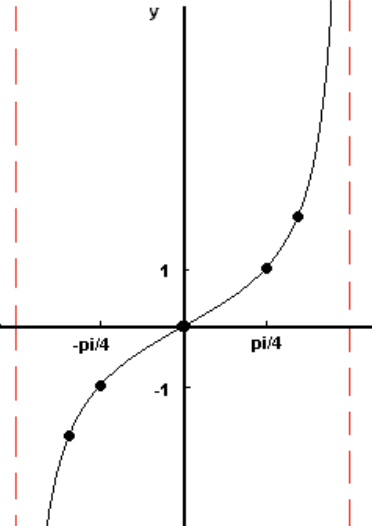
\includegraphics[width=3cm]{week1_wednesday}
\caption{Graph of solution}
\end{figure}
There is ``nothing'' outside $\frac{\pi}{2}$. In fact, there might be some graph satisfied the equation. However, it is non-sense because we can not specify the value of $y(t)$ outside $\frac{\pi}{2}$.
\item[[2]] See definition of {\it direction field} in text book.

\end{itemize}
\end{remark}
\begin{example}

\[
\left \{	\begin{gathered}
y^\prime=1+y^2 	\\
y(0)=1
\end{gathered}	\right.
\]
$\Rightarrow$\qquad\dots$y=\tan(t+c)$\qquad$1=y(0)=\tan c$ $\Rightarrow$ $c=\frac{\pi}{4}+k\pi$\\
\[y=\tan(t+\frac{\pi}{4})\]
\end{example}
[Difference equation of the example 1.2]\[\frac{y(t_2)-y(t_1)}{t_2-t_1}=1+y^2(t_1)
\]\\Difference equation can be used to approximate the behaviour of the solution of DE.
Take $t_2=t_1+1$, $y(0)=0, y(1)=1, y(2)=3, y(3)=13, y(4)=183,\dots$, we roughly guess the behaviour of $y(t)$. Although, this is not quite accurate.
\subsection{Population method}
$P(t):$ total population at time $t$.\\
$r(t,p)$: growth rate (birthrate-death rate)\\
Malthus theory: $\frac{1}{p}\frac{\diff p}{\diff t}=r$
 is a constant. (The differentiation of population by time $\frac{\diff p}{\diff t}$ is $rp$)
\[lnp=rt+c\]
\[p(t)=e^ce^{rt}=\tilde{c}e^{rt}
\]
\[p(t)=p(0)e^{rt}
\]
This is imposible considering the limited nature resource.\\
\emph{Logistic equation}(Verhulst 1837)\\
$\left \{	\begin{gathered}
p^{\prime}=p(a-bp)	\\
p(0)=p_0
\end{gathered}\right.$
\[\int\frac{\diff p}{p(a-bp)}=\int\diff t=t+c
\]
To integrate left-hand side, we need a little trick:
\[\frac{1}{p(a-bp)}=\frac{A}{p}+\frac{B}{a-bp}
\]
\[
\begin{aligned}
	 \frac{1}{p(a-bp)}&=\frac{A}{p}+\frac{B}{a-bp}  \\
 		&=\frac{aA+(B-bA)p}{p(a-bp)}\\	
\end{aligned}
\]
$\Rightarrow$ $A=\frac{1}{a}$, $B=\frac{b}{a}$
\[
\begin{aligned}
	 \int\frac{\diff p}{p(a-bp)}&=\frac{1}{a}\int\frac{1}{p}\diff p+\frac{b}{a}\int\frac{\diff p}{a-bp}=t+c  \\
 		&=\frac{1}{a}lnp-\frac{1}{a}ln|a-bp|=\frac{1}{a}ln\frac{p}{|a-bp|}\\	
\end{aligned}
\]
\[\boxed{\frac{p}{|a-bp|}=\tilde{c}e^{at}, \tilde{c}>0}\]





